\section{STM32}

\subsection{Nov 04, 2021}

CubeIDE vs CubeMX differences?
\\add path trong environments, edit file path, link to the folder store the make (cygwin), git, etc. so we could use it in the terminal of the visual code.


\subsection{Nov 05, 2021}
Equivalences at tstamp 7:15

reference nhung noi de thay doi file makefile tuy theo loai chip trong video 02 - toanchung

\subsection{Nov 29, 2021}

Compare JTAG vs SWD
The other good thing about SWD is you can use the serial wire viewer for your printf statements for debugging.
\begin{figure}[h]
  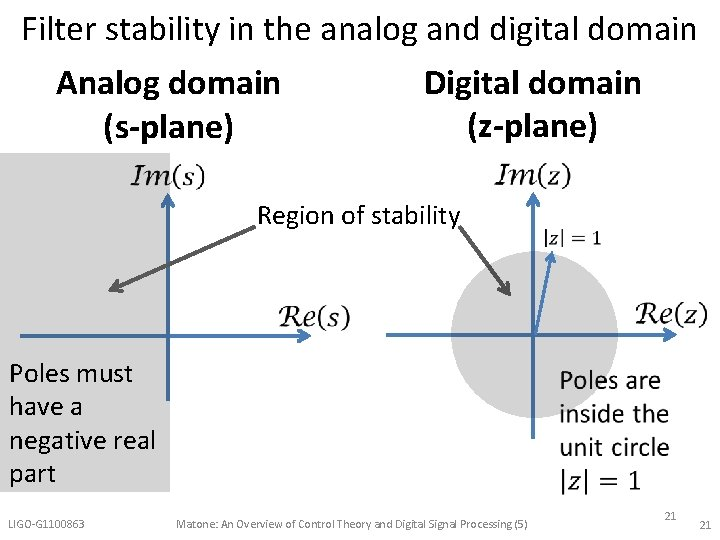
\includegraphics[scale=0.3]{control_bootcamp_stable_region_in_s_and_z_domain}
  \caption{Mapping stable region between s-continuos and z-discrete domain}  
\end{figure}

\section{C - PROGRAMMING}
Pointers\\
array[ ] different ? is it a 2 dimension, 3 dimensions array?\\
int * const array, use array name, so it is 1 dimension (single subscripted array?)\\
what is the principle of least privilege?
opreands la gi?\\
Portability Tip 7.3\\
Most computers today have 2-byte or 4-byte integers. Some of the newer machines use 8-
byte integers. Because the results of pointer arithmetic depend on the size of the objects a
pointer points to, pointer arithmetic is machine dependent.\\
Pointers are valid operands in arithmetic expressions, assignment expressions and comparison expressions.\\
Arithmetic operations: cac phep tinh toan hoc, basics: + - x / 
\\
how to know the system is 2, 4 or 8 byte systems?
\\
Pointers can be compared using equality and relational operators, but such comparisons are meaningless unless the pointers point to elements of the same array
\\
Array element b[3] can alternatively be referenced with the pointer expression: *( bPtr + 3 )\\
The parentheses are necessary because the precedence of * is higher than the precedence of + .
\\
string vs character array?\\
What is the end char of the string? null? "'slash 0'?" how to see it?\\
const int * xPtr \\
int * const xPtr \\
const char * const s2\\
\\DESIGN STEP
\\first think about the flow of the codes
\\which variable is fixed, should not be changed by mistakes, then use the qualifier const
\\should only pass the variable by value and return ONLY ONE value in each function for the principle of least of privilege
\\should not change the value of the variable inside the function if you dont really need to do that

%\begin{figure}[h!]
%    \centering
%    \includegraphics[scale=1.7]{universe}
%    \caption{The Universe}
%    \label{fig:universe}
%\end{figure}